
A world is easily divided into different aspects. There are the sky, the oceans and the land. The land contain different terrain, with different types of ground and vegetation. There is a sun orbiting the world, casting rays of light and in the process creating reflections and indirectly making shadows.\\
\\
A procedural world is generated by carefully chosen algorithms. Our world is procedurally generated anew in a new unique constellation on every run, or a seed can be provided to generate specific worlds. The terrain is first formed, then the ground texturing and the vegetation, both dependent on properties of the terrain. The shadows depend on the sun and the waves on the terrain as well as on time itself.

\subsubsection{Sky}
The sky is achieved using a high-resolution texture of a sky mapped to a skybox. The mathematical location of the sun is placed as close as possible to the sun appearing in this texture. This gives shadows and shading a natural feel. The texture has been manually modified at the horizon to fade towards a shadowish gray color. The color is the same as the one objects are distance-fogged with. This makes the sky melt into the ocean in a very nice way. 

\subsubsection{Ocean}
The water is made up of a normal-mapped square and a blue color. The normal map is repeated over the square and is moving in texture space, giving the illusion of a wind. The normal map movement cycles such that when the water normal map has been totally displaced, it starts over again from its original position. This movement makes the water glitter from a far, see figure \ref{fig:water}.
\begin{figure}[H]
\begin{subfigure}{.5\textwidth}
  \centering
  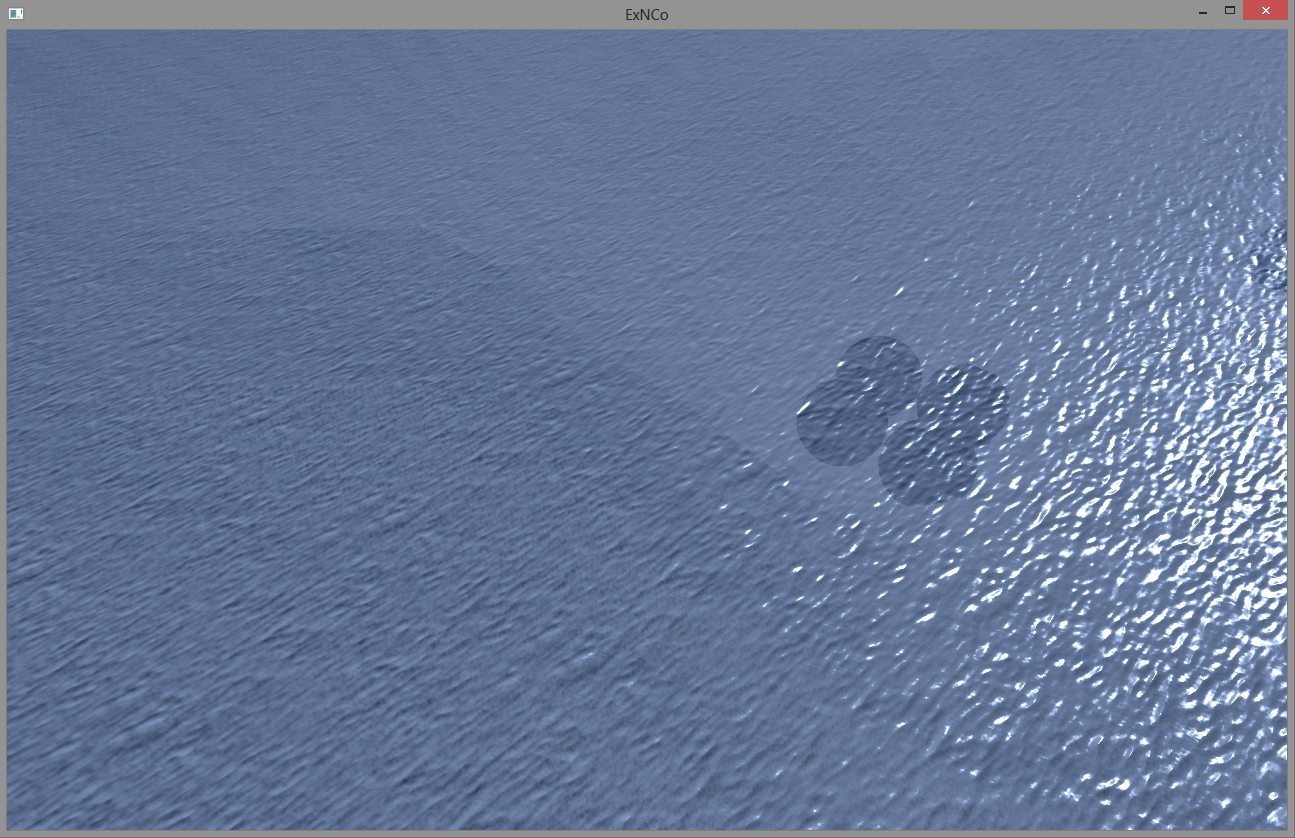
\includegraphics[width=0.9\linewidth]{images/waterWaves.png}
  \caption{The water.}
  \label{fig:waterWaves}
\end{subfigure}%
\begin{subfigure}{.5\textwidth}
  \centering
  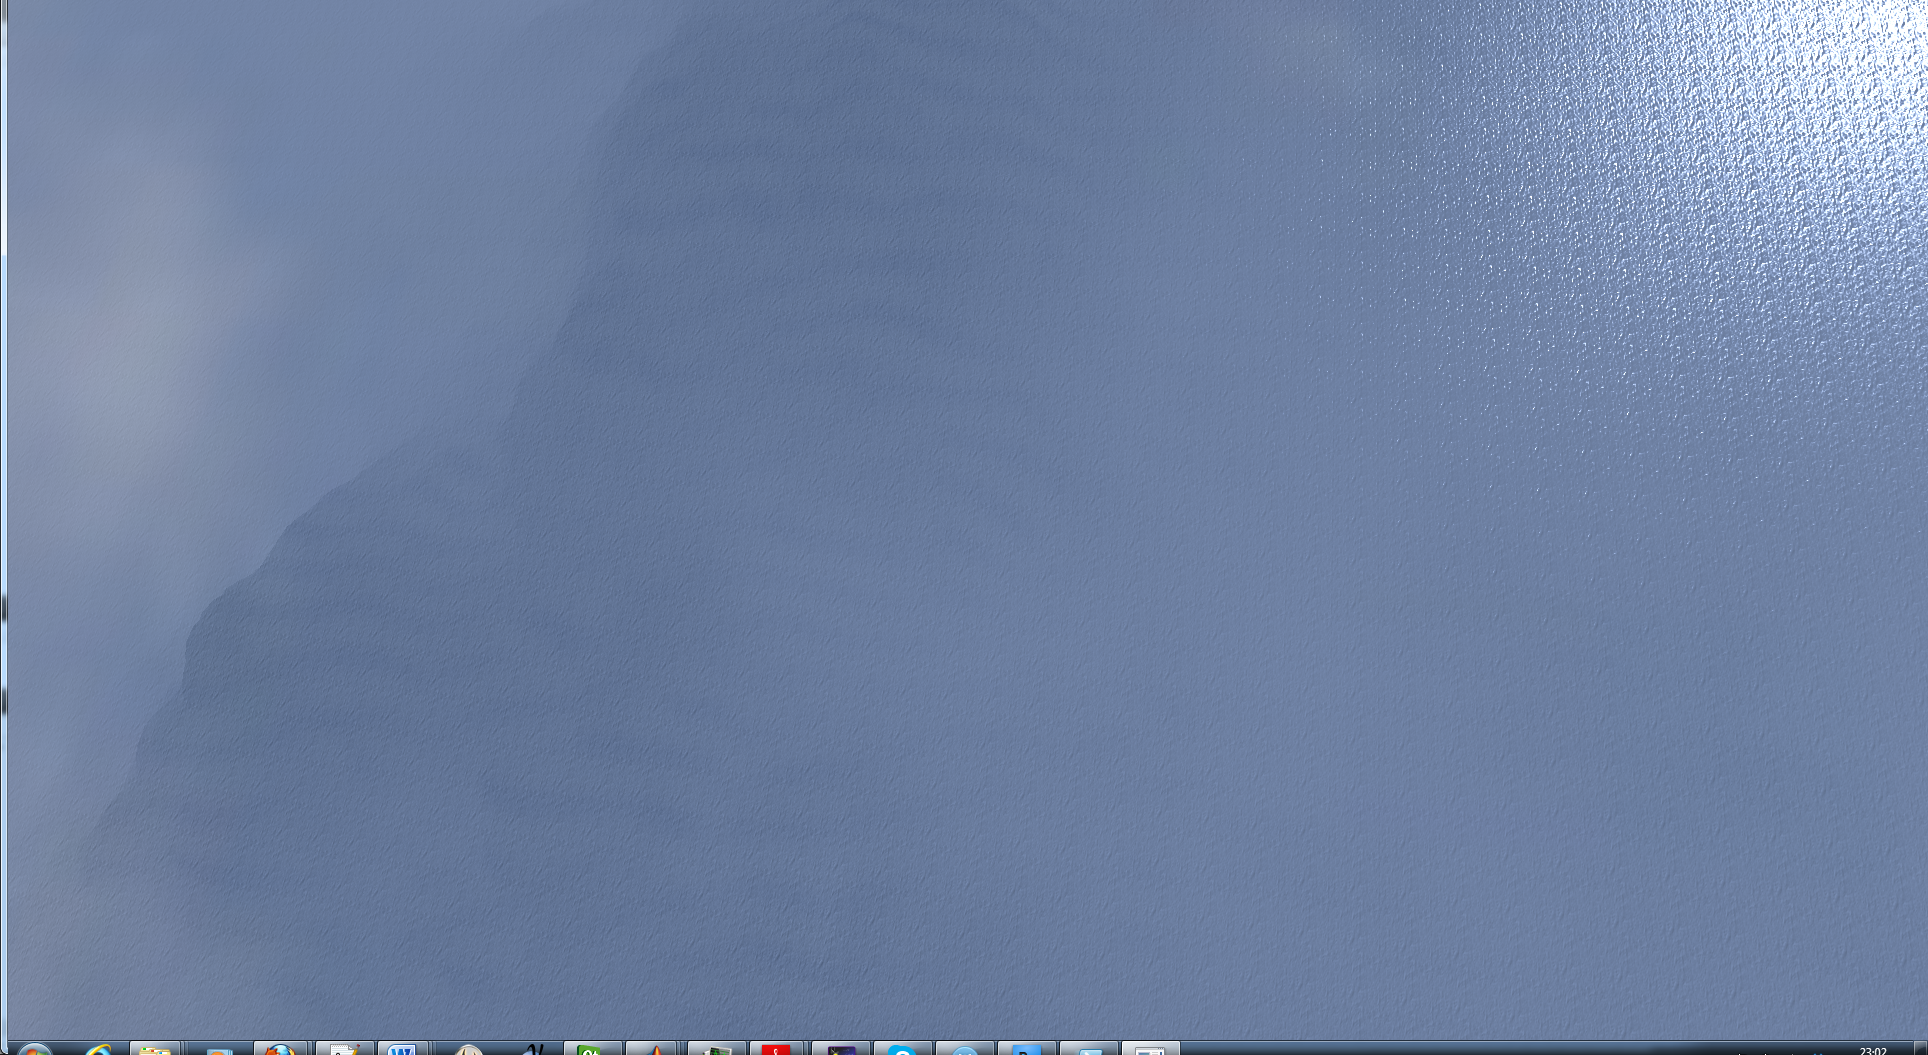
\includegraphics[width=0.9\linewidth]{images/waterGlimmer.png}
  \caption{Glittering water.}
  \label{fig:waterGlistering}
\end{subfigure}
\caption[Noise comparison]{\textit{Comparison of noise functions}}
\label{fig:water}
\end{figure}
Waves on the beaches is made by having several sinus waves aggregate horizontally to vary the wave fronts, and by having a sinus wave that control the vertical assent/decent of the waves. It is hard to catch on a screen shot, but an image of the waves in the world is shown in figure \ref{fig:waves}
\begin{figure}[H]
  \centering
  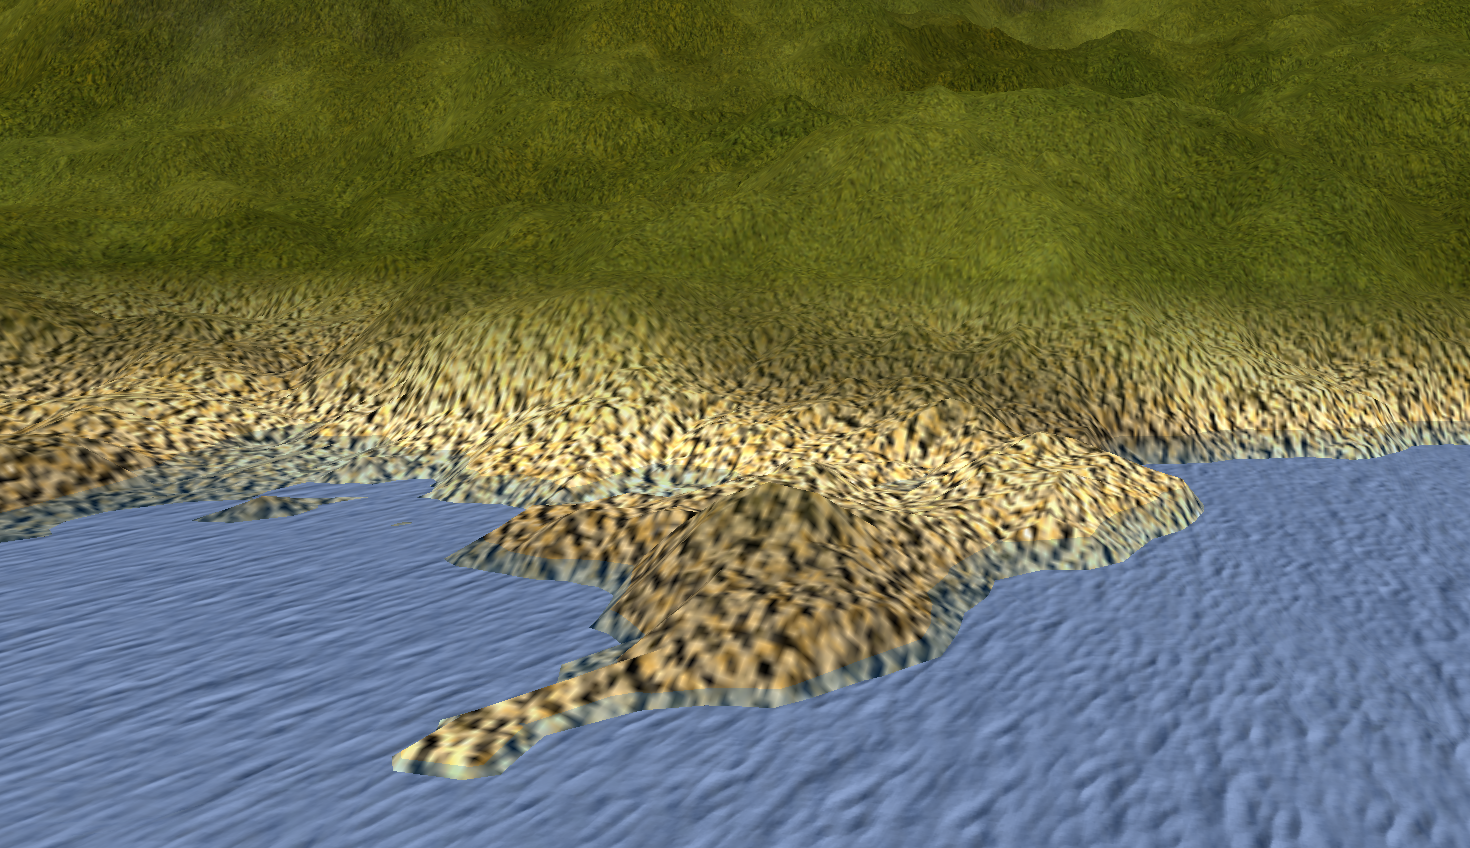
\includegraphics[width=0.9\linewidth]{images/waves.png}
  \caption{The waves are seen at the beach.}
  \label{fig:waves}
\end{figure}%
The sky is reflected in the water by using an image which is the projection of the sky onto the ocean as a texture for the water. This texture is moving with the camera in the xz-plane. An example is seen in figure \ref{fig:skyReflection}. It could be improved in the future by taking the height of the camera in consideration as well, or to continuously project the sky onto the water according to the camera position. Currently the camera height do not change the reflection, making it unrealistic if moving up and down.
\begin{figure}[H]
  \centering
  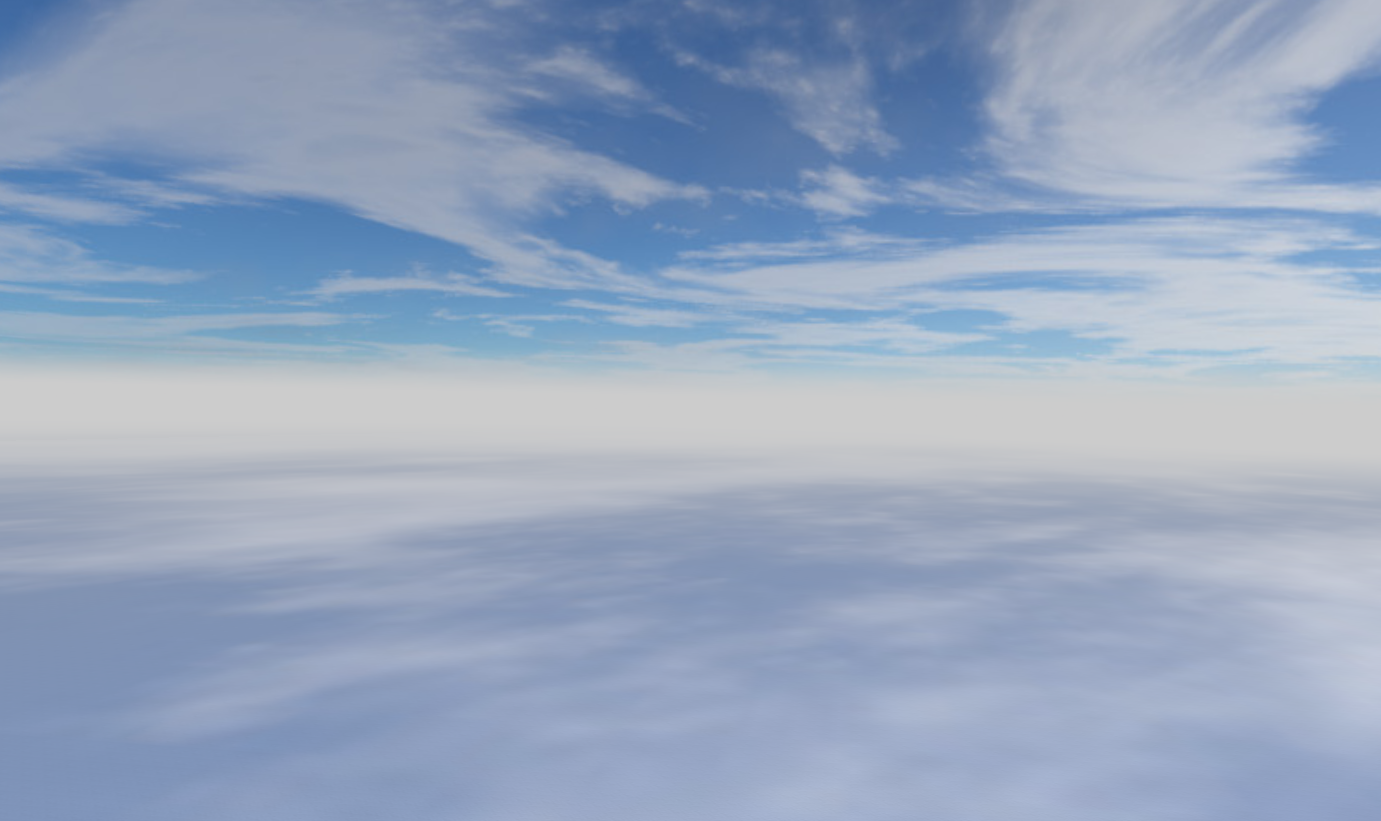
\includegraphics[width=0.9\linewidth]{images/reflectingSky.png}
  \caption{The sky reflected in the ocean.}
  \label{fig:skyReflection}
\end{figure}%

\newpage
\subsubsection{Terrain}
The terrain is generated by sampling a noise function and translating its value into a height for the current vertex. The noise in this case originates from a Simplex function. However, to get a realistically looking terrain one it is not sufficient to sample this function only once for every vertex.

Fractional Brownian Motion is calculated by sampling the Simplex function at different frequencies and calculating a weighted sum over the samples \cite{FracBrownMotion}.  The result is a nice looking height map. 

\begin{figure}[H]
\begin{subfigure}{.5\textwidth}
  \centering
  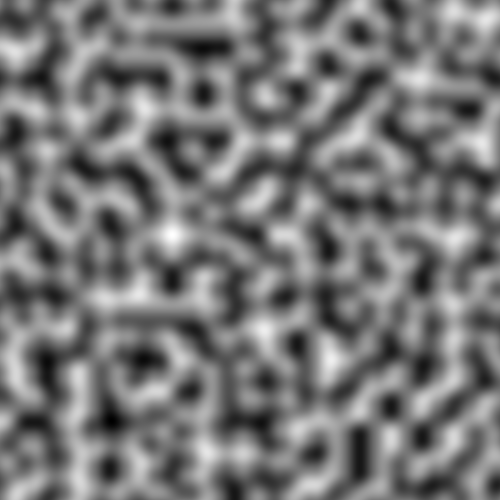
\includegraphics[width=0.9\linewidth]{images/Simplex.png}
  \caption{Height map generated from single-octave simplex noise}
  \label{fig:sub1}
\end{subfigure}%
\begin{subfigure}{.5\textwidth}
  \centering
  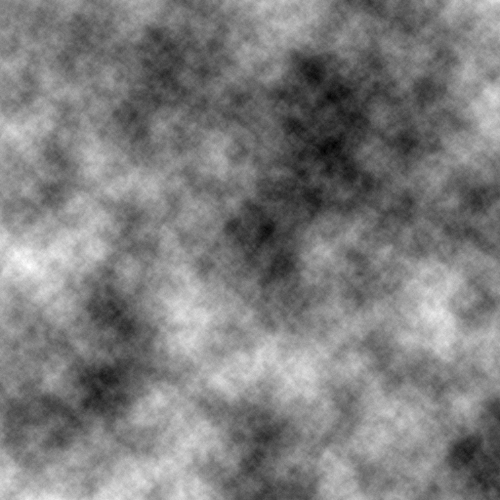
\includegraphics[width=0.9\linewidth]{images/FracBrownMotion.png}
  \caption{Height map generated with Fractional Brownian Motion}
  \label{fig:sub2}
\end{subfigure}
\caption[Noise comparison]{\textit{Comparison of noise functions}}
\label{fig:R_kitchen_example}
\end{figure}

\subsubsection{Ground}
The ground is textured using a non-linear multi-texturing approach based on both altitude and terrain slope. Currently only three textures are used, one sandy, one grassy and one rocky. ... TODO: blah...\\
\\
FIGURE(comparison of texturing)
\\
FIGURE(comparison of texturing)
\\
\begin{figure}[H]
\begin{subfigure}{.5\textwidth}
  \centering
  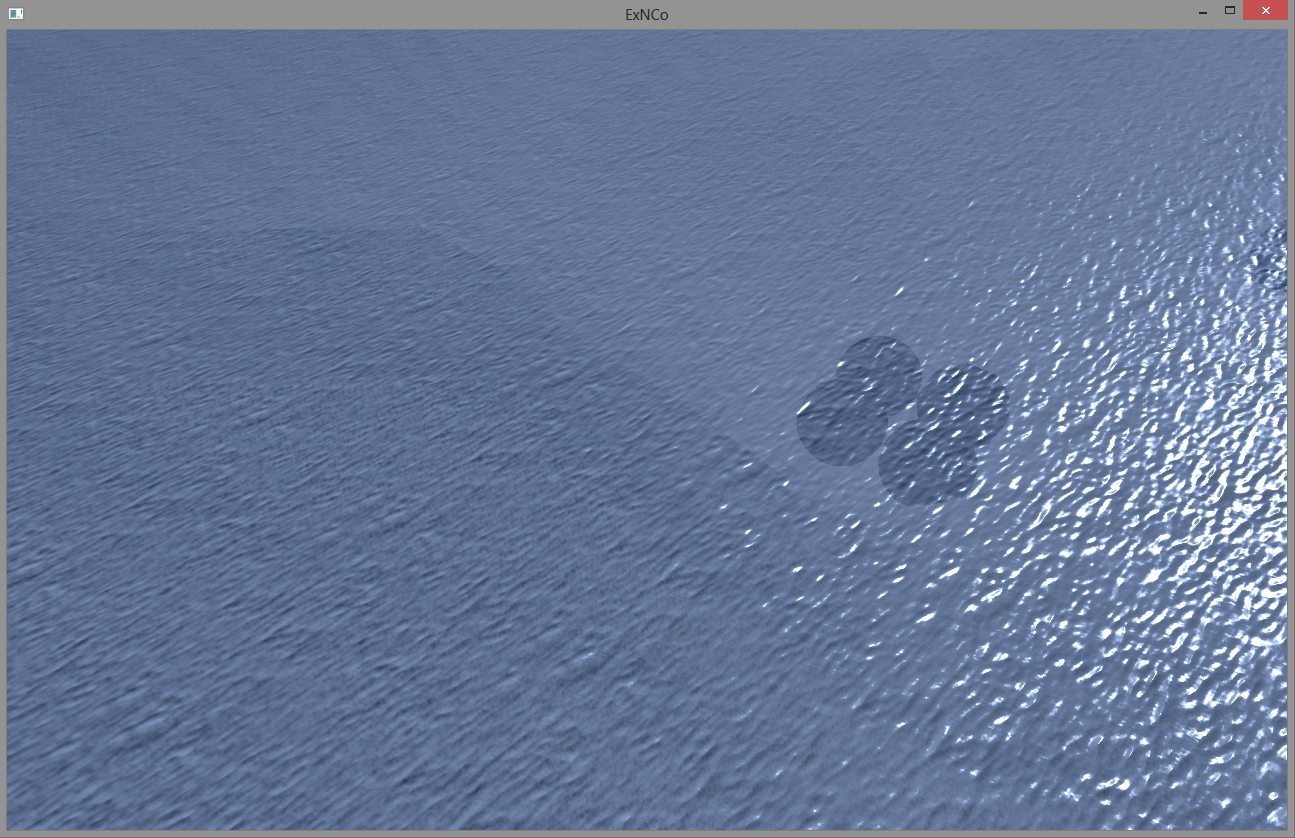
\includegraphics[width=0.9\linewidth]{images/waterWaves.png}
  \caption{The water.}
  \label{fig:waterWaves}
\end{subfigure}%
\begin{subfigure}{.5\textwidth}
  \centering
  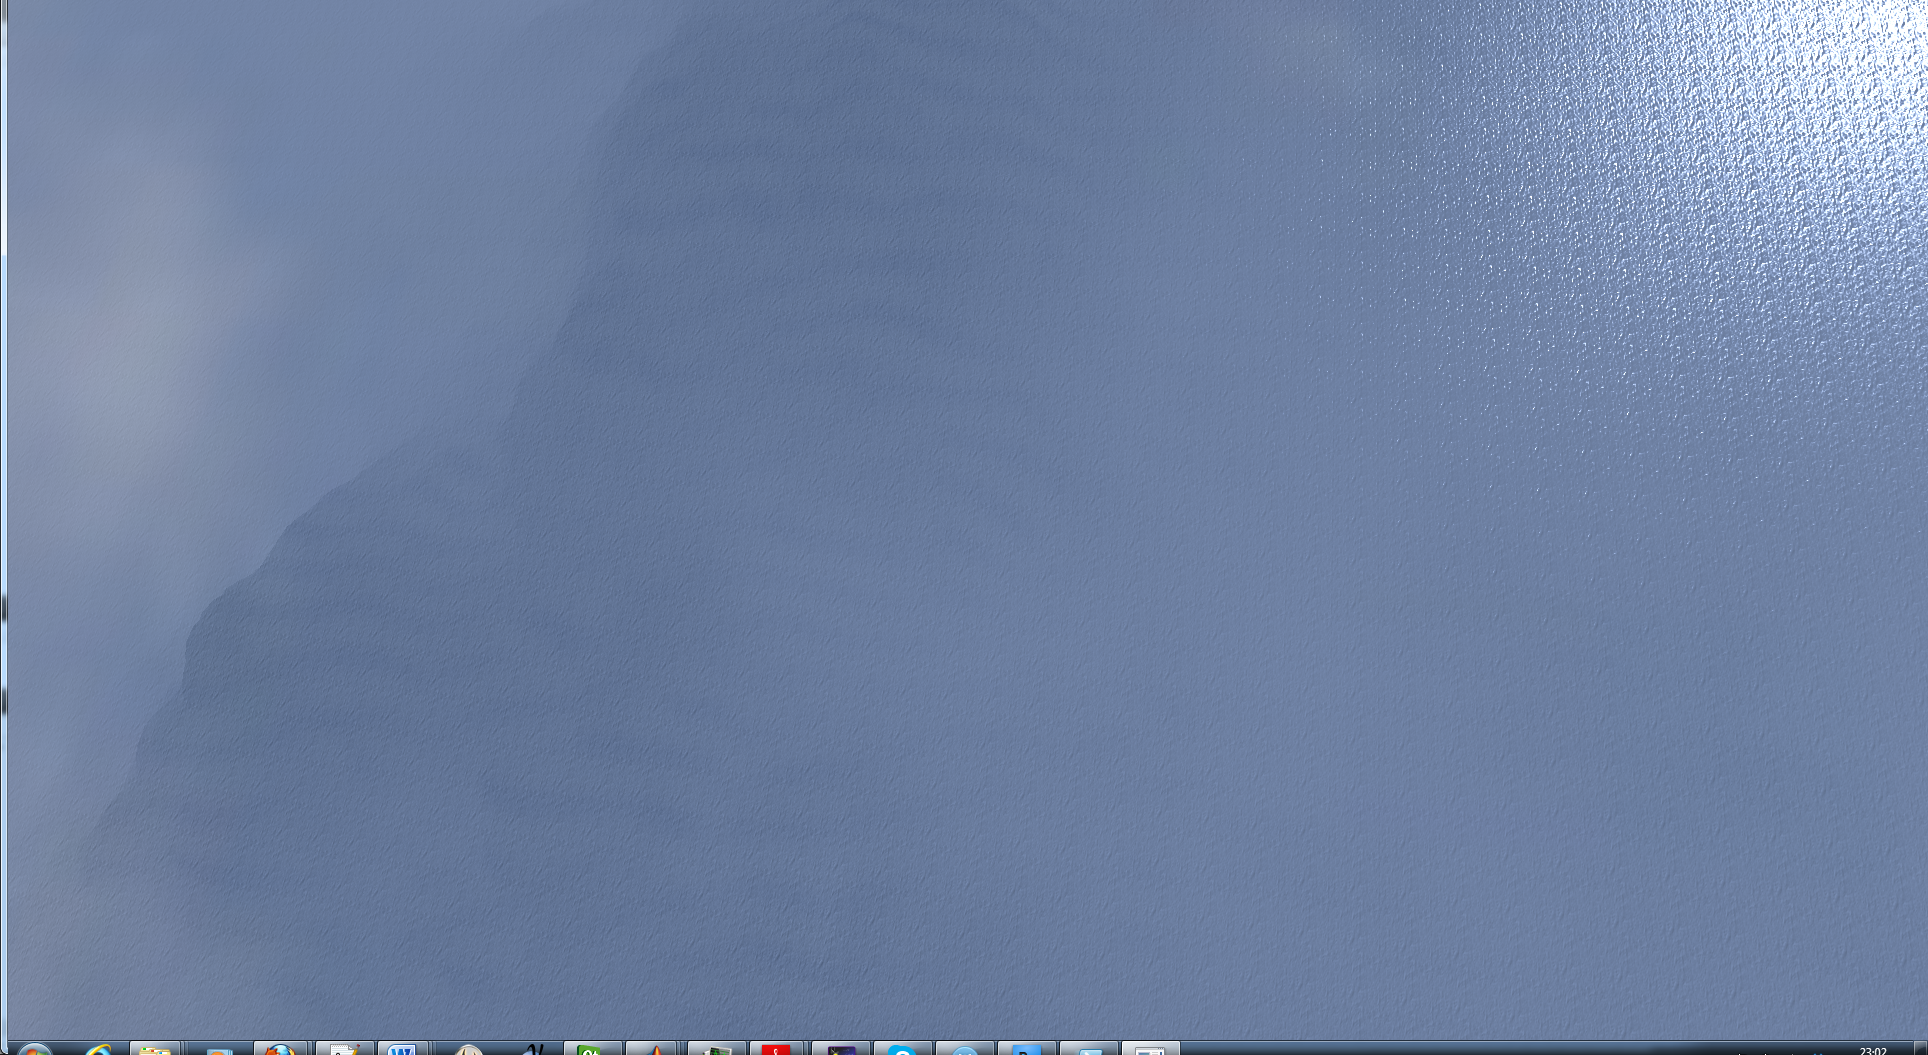
\includegraphics[width=0.9\linewidth]{images/waterGlimmer.png}
  \caption{Glittering water.}
  \label{fig:waterGlistering}
\end{subfigure}
\begin{subfigure}{.5\textwidth}
  \centering
  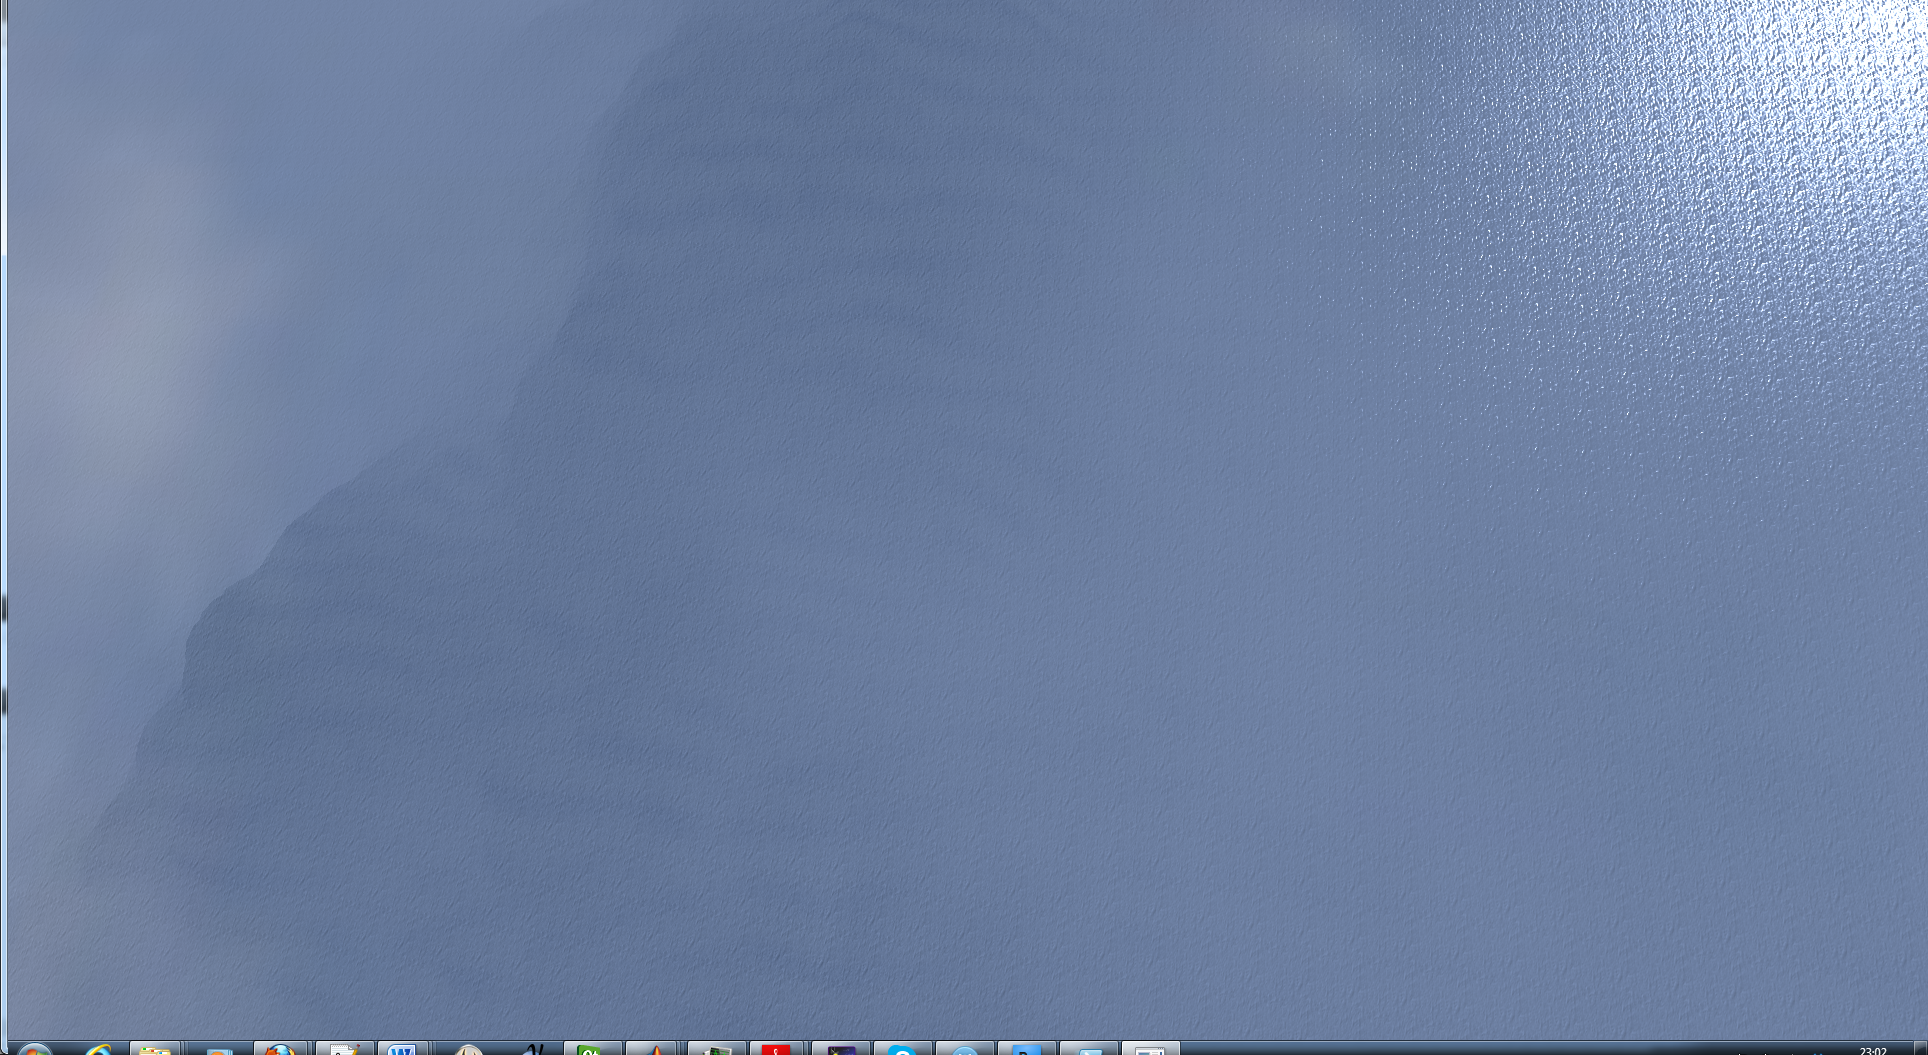
\includegraphics[width=0.9\linewidth]{images/waterGlimmer.png}
  \caption{Glittering water.}
  \label{fig:waterGlistering}
\end{subfigure}
\caption[Noise comparison]{\textit{Comparison of noise functions}}
\label{fig:water}
\end{figure}

\subsubsection{Content}
// TODO - Häger \\
Trees and rocks 
\begin{figure}[H]
  \centering
  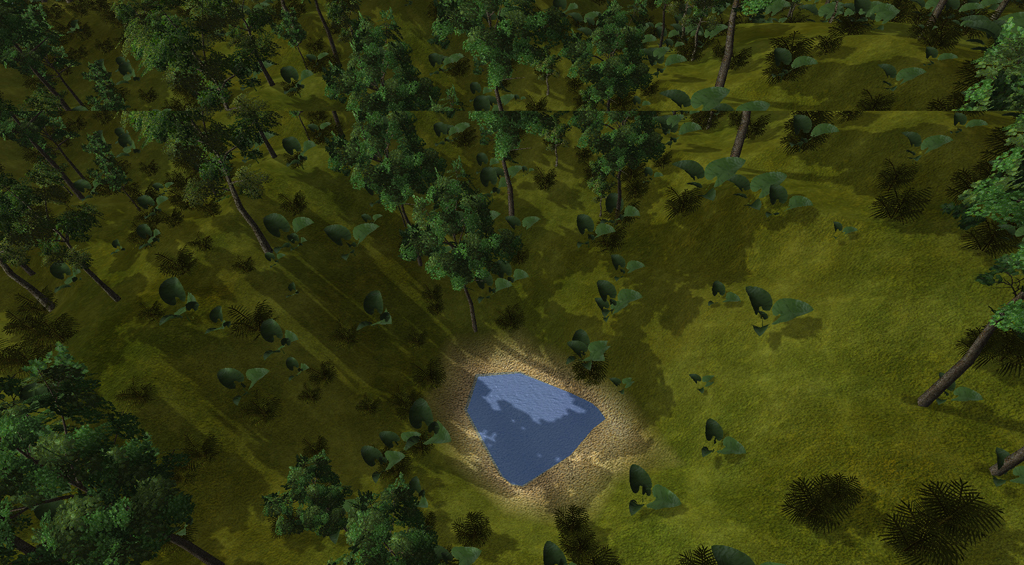
\includegraphics[width=0.9\linewidth]{images/content1.eps}
  \caption{A small water hole in the middle of the forest at the late afternoon.}
  \label{fig:water_hole}
\end{figure}%

\subsubsection{Volcano}
\begin{figure}[H]
  \centering
  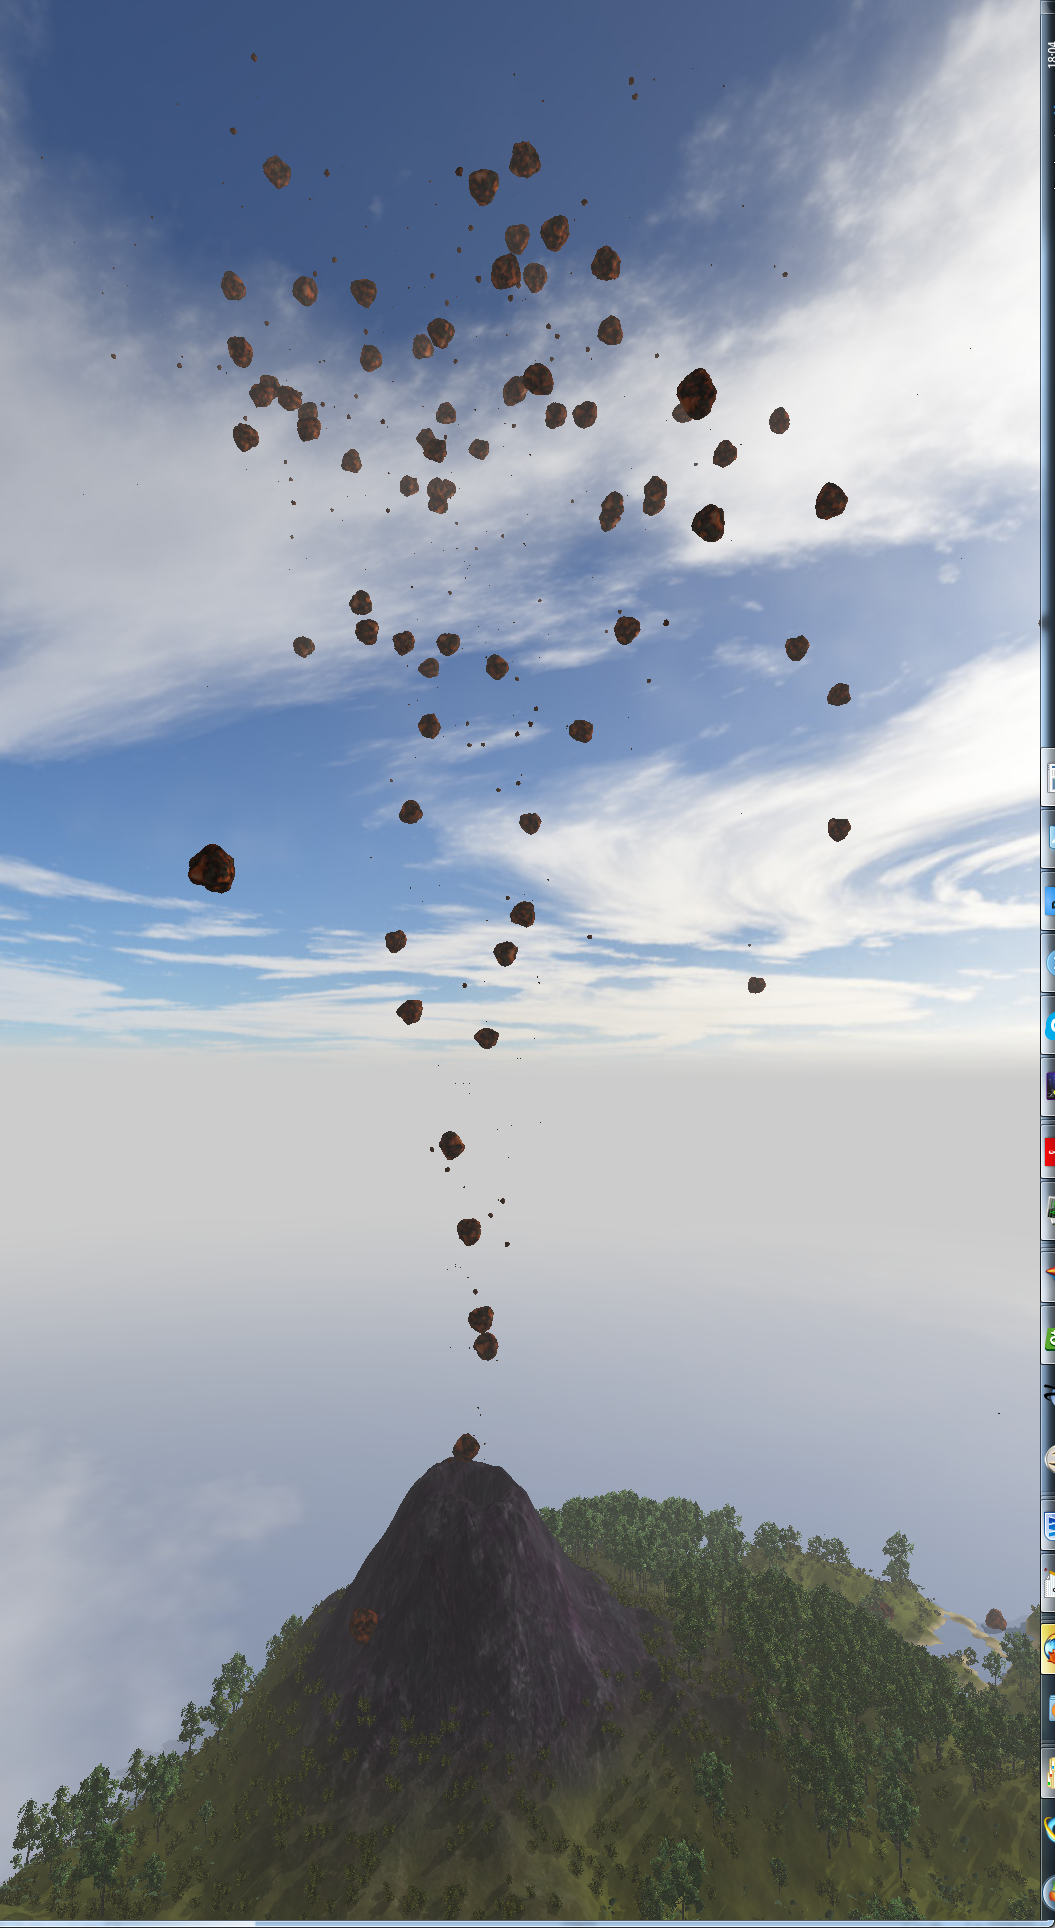
\includegraphics[width=0.8\linewidth]{images/volcano.png}
  \caption{A vulcano.}
  \label{fig:vulcano}
\end{figure}%
// TODO - Tigerwra\\
\\
The volcano is made up of the addition and the subtraction..\\
\\
When the fire balls enter the water and sink too deep, they are re-spawned in the volcano and sent out though the hole again.
\\
\\
The physics can be reversed in time, and balls returning to the volcano hole is then placed where they were when they disappeared, with all the physical properties reset to how they were at that time as well.
\\
\begin{figure}[H]
\begin{subfigure}{\textwidth}
  \centering
  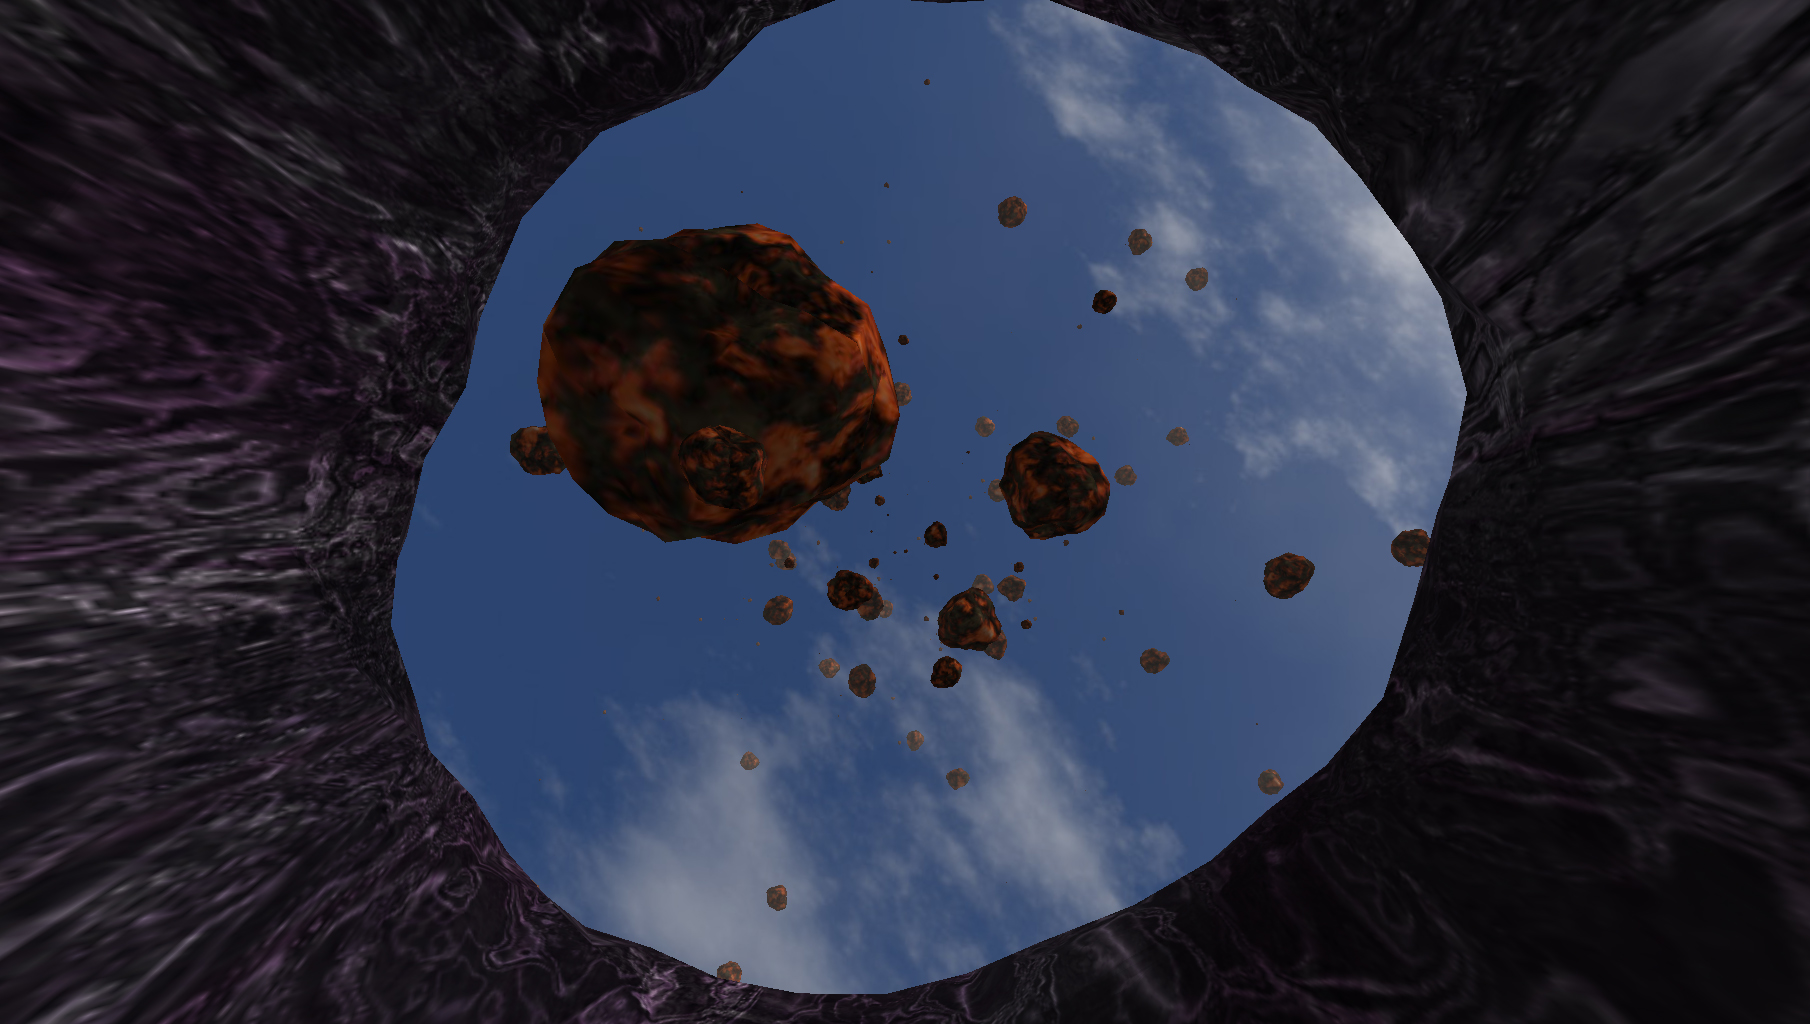
\includegraphics[width=0.9\linewidth]{images/Volcano1.eps}
  \caption{...}
  \label{fig:vulcano1}
\end{subfigure}%
\\
\begin{subfigure}{\textwidth}
  \centering
  \includegraphics[width=0.9\linewidth]{images/Volcano2.eps}
  \caption{...}
  \label{fig:vulcano2}
\end{subfigure}
\caption[Noise comparison]{\textit{Volcano eruption.}}
\label{fig:vulcano3}
\end{figure}



